\section{AdaPlanBench Construction}

\BENCH{} is a dynamic, interactive benchmark for evaluating agents' adaptive planning under dual constraints, rooted in household tasks where both world and user constraints naturally arise~\citep{chang2024partnrbenchmarkplanningreasoning}.
% \xiusi{Here: for each step below, it would be better to first highlight the motivation and goal (what we want to achieve and why) before illustrating the procedure (how). This version only has the latter, so the reviewer may find it hard to follow.}
% Built on the MacGyver dataset~\citep{MacGyver}, it augments each instance with both world and user constraints through an automatic, scalable pipeline.
% These constraints are revealed progressively during interaction: whenever an agent proposes a plan that violates a hidden requirement, that constraint is disclosed, thus requiring the agent to adaptively re-plan.
As illustrated in Figure~\ref{fig:overview}, AdaPlanBench consists of two tightly coupled parts: an automatic pipeline that constructs world and user constraints for each MacGyver query, and a runtime protocol that progressively reveals violated constraints to elicit adaptive re-planning. 
This setting poses a distinctive challenge for agents, which must infer latent constraints from partial feedback, keep track of previously disclosed violations, and continuously revise their plans under an evolving constraint set.
As shown in \Cref{tab:comparison-table}, \BENCH{} distinguishes itself from prior work by focusing on interactive planning under both user and world constraints.
We discuss related work and the significance of this setting further in Appendix~\ref{app:related-works} and~\ref{app:discussion-significance-generalization}.


\begin{figure}
    % \vspace{-10mm}
    \centering
    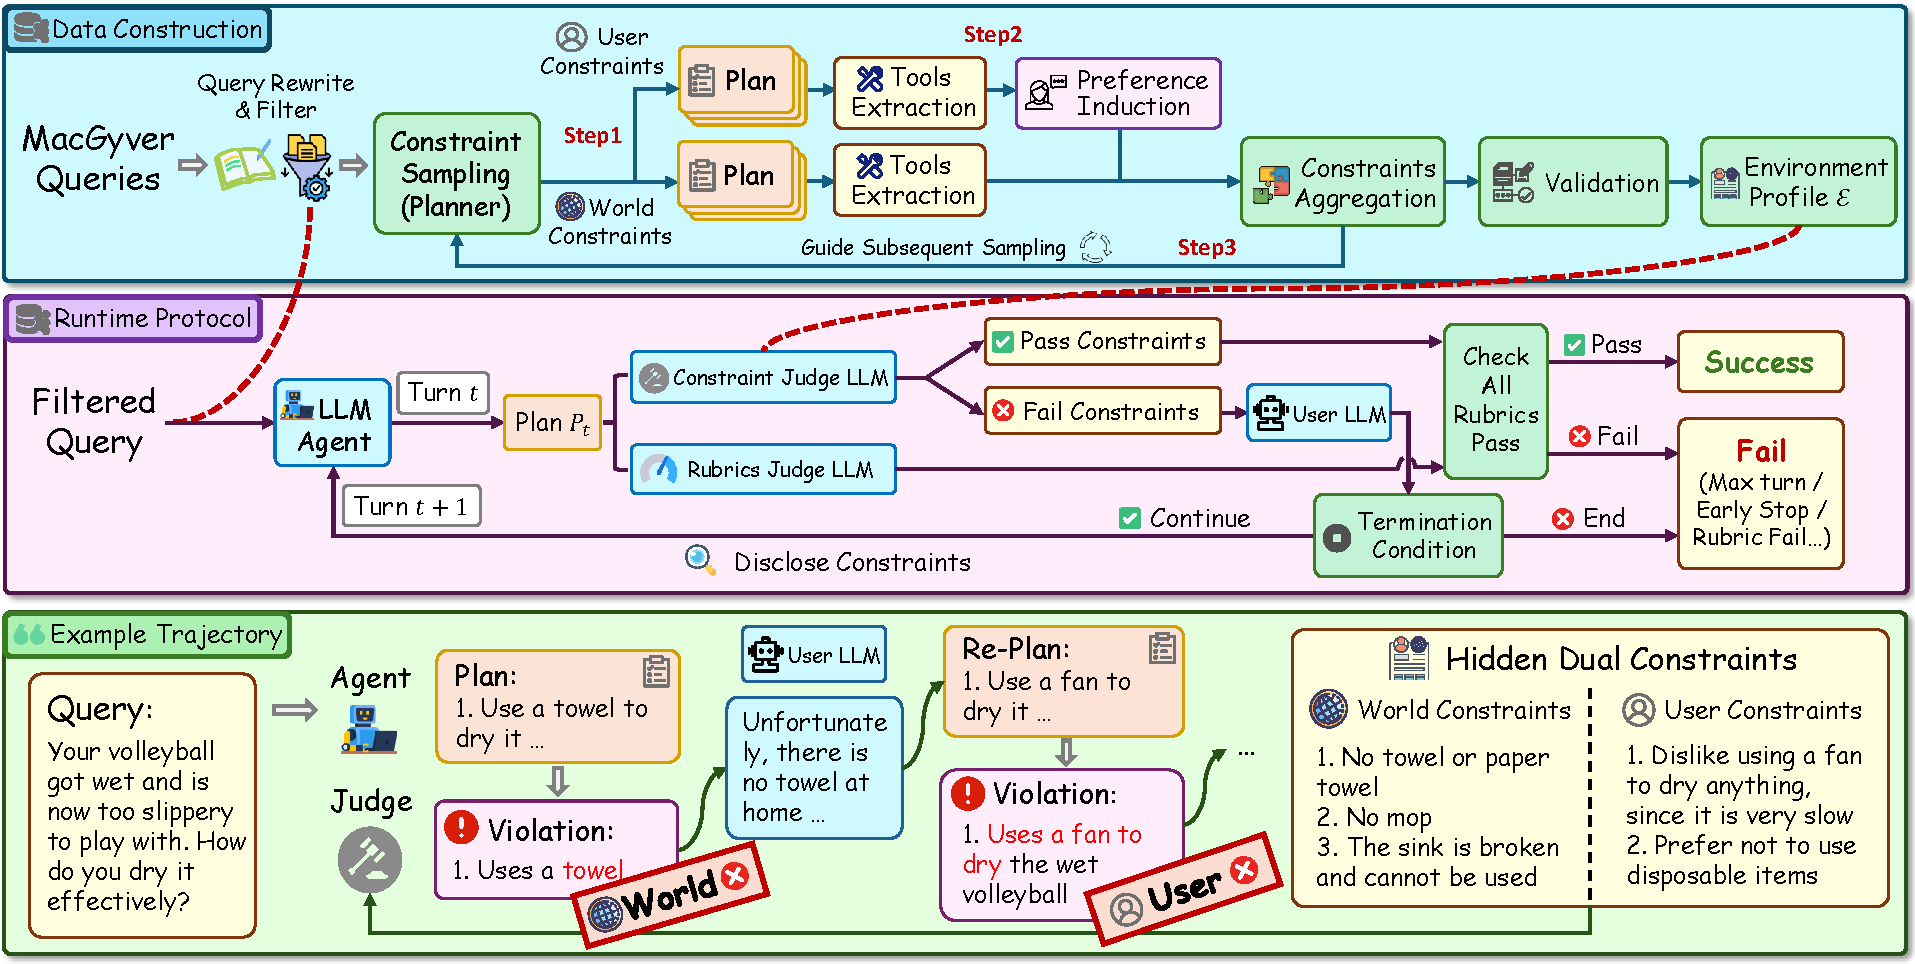
\includegraphics[width=\linewidth]{figures/pipeline_1.pdf}
    \vspace{-0.2in}
    \caption{Overview of AdaPlanBench. \textit{Top}: data construction, where dual constraints are constructed for each query. \textit{Middle}: runtime interaction, where the agent proposes plans, receives feedback on violated constraints, and re-plans iteratively. \textit{Bottom}: an example trajectory showing how hidden constraints are progressively disclosed during interaction.
    }
    \label{fig:overview}
    \vspace{-4mm}
\end{figure}

\subsection{Data Construction}
\label{sec:data-construction}
To construct each benchmark instance, we first rewrite and filter raw MacGyver queries, and then build a dual-constraint profile for each retained query using a multi-agent framework.
For each filtered query from MacGyver, we construct a dual-constraint profile using a multi-agent framework with specialized components. Formally, each instance is mapped to $(q,\mathcal{E})$, where $q$ is the query and $\mathcal{E}=(\mathcal{B}_{w},\mathcal{B}_{u})$ is the resulting constraint profile, comprising a world constraint set $\mathcal{B}_{w}$ and a user constraint set $\mathcal{B}_{u}$. The framework uses a set of role-specific models \{${\mathcal{M}_{\mathrm{rw}}, \mathcal{M}_{\mathrm{flt}}, \mathcal{M}_{\mathrm{plan}}, \mathcal{M}_{\mathrm{ext}}, \mathcal{M}_{\mathrm{merge}}, \mathcal{M}_{\mathrm{chk}}}$\}, which respectively denote a query rewriter, a binary query filter, a set of planner samplers, a constraint extractor, a merge model, and a constraint checker. Model choice details are provided in Appendix~\ref{app:model_choise}.

\noindent\textbf{Query rewriting and filtering.}
For each raw MacGyver query $q^{\mathrm{raw}}$, we first use the rewriter $\mathcal{M}_{\mathrm{rw}}$ to produce a short, method-agnostic household query {\small $q=\mathcal{M}_{\mathrm{rw}}(q^{\mathrm{raw}})$} by removing explicit resource constraints (e.g., \textit{tools available: ...} or \textit{using only ...}) while preserving the original goal. We then apply a strict binary filter $\mathcal{M}_{\mathrm{flt}}$ to retain only concrete household tasks that require multi-step planning. 
Because this process relaxes only the original resource constraints, we preserve the corresponding MacGyver reference solution for each retained query and use it later for constraint extraction and validation, thus ensuring task solvability. 
Detailed filtering rules are provided in Appendix~\ref{app:data_filtering_rule_exp} and illustrated in \Cref{fig:filtering_rules}.

To construct the dual-constraint profile, we iteratively repeat three steps: (1) sample candidate plans for the task, (2) extract salient tools from the plans and convert them into world or user constraints, and (3) merge the constraints to guide the next round of sampling.

\noindent\textbf{Step 1: Plan sampling.}
We first sample diverse candidate plans to surface the tools and strategies that are likely to matter for the task.
We employ a family of $J$ planner samplers {\small $\{\mathcal{M}^{(j)}_{\mathrm{plan}}\}_{j=1}^{J}$} and run the procedure for at most $R$ rounds, yielding a sequence of progressively enriched constraint profiles $\mathcal{E}_{low}, \mathcal{E}_{mid}, \mathcal{E}_{high}$. At each round $r$, every planner samples plans:
\begin{footnotesize}
\begin{equation}
\pi^{(j)}_{r} = \mathcal{M}^{(j)}_{\mathrm{plan}}\!\left(q,\mathcal{B}^{(j)}_{w,r-1},\mathcal{B}^{(j)}_{u,r-1}\right),
\end{equation}
\end{footnotesize}
where {\small $\mathcal{B}^{(j)}_{w,r-1}$} and {\small $\mathcal{B}^{(j)}_{u,r-1}$} denote the world and user constraint pools accumulated for planner $j$ up to round $r-1$, respectively. Both pools are initialized as empty sets. Intuitively, {\small $\mathcal{B}^{(j)}_{w,r-1}$} records world constraints such as unavailable tools or environmental limitations that subsequent plans must respect, while {\small $\mathcal{B}^{(j)}_{u,r-1}$} records user constraints such as preferences or requirements that later plans should not violate.

\noindent\textbf{Step 2: Constraint extraction.}
We then transform tools and their usage in these plans into grounded world and user constraints.
In our benchmark, world constraints capture tool availability and usability in the environment, whereas user constraints capture whether the tools used in a plan, or the attributes implied by their use, align with user preferences. This abstraction is designed to preserve both groundedness and evaluability (see Appendix~\ref{app:user-attribute-discussion}).

Given a sampled plan {\small $\pi^{(j)}_{r}$}, we first use $\mathcal{M}_{\mathrm{ext}}$ to extract the tools used in the plan:
\begin{footnotesize}
\begin{equation}
\mathcal{T}^{(j)}_{r} = \mathcal{M}_{\mathrm{ext}}(q, \pi^{(j)}_{r})
\end{equation}
\end{footnotesize}
These extracted tools form the raw basis for constraint construction. We then derive world and user constraints from them respectively as follows:
\begin{itemize}[topsep=-1.5pt, leftmargin=10pt, itemsep=0pt]
\item For \textbf{world constraints}, we directly convert each extracted tool into a constraint candidate {\small $\mathcal{C}^{(j)}_{w,r}$} by restricting its availability or use. For example, for the query of removing wrinkles from a suit, a world constraint could be \textit{there is no iron at home}.
% \item For \textbf{user constraints}, we use $\mathcal{M}_{\mathrm{ext}}$ to further infer attributes tool or its usage that may matter to the user, and then formulate corresponding constraint candidates {\small $\mathcal{C}^{(j)}_{u,r} \sim \mathcal{M}_{\mathrm{ext}}(q, \mathcal{T}^{(j)}_{r})$}. 
\item For \textbf{user constraints}, we use $\mathcal{M}_{\mathrm{ext}}$ to further infer attributes of tools or their usage that may matter to the user, and then formulate corresponding constraint candidates {\small $\mathcal{C}^{(j)}_{u,r} \sim \mathcal{M}_{\mathrm{ext}}(q, \mathcal{T}^{(j)}_{r})$}.
For the same example, a user constraint could be \textit{I am concerned about using tools that generate high heat}, where \textit{generate high heat} is the inferred attribute associated with the tool \textit{iron}.
\end{itemize}

\noindent\textbf{Step 3: Constraint merging.}
Finally, we merge and canonicalize discovered constraints so they can reliably guide later rounds of planning.
After extraction, we use $\mathcal{M}_{\mathrm{merge}}$ to combine newly generated constraints with the previously accumulated ones, canonicalizing and deduplicating them to maintain a consistent representation:
\begin{footnotesize}
\begin{equation}
\mathcal{B}^{(j)}_{w,r} = \mathcal{M}_{\mathrm{merge}}(\mathcal{B}^{(j)}_{w,r-1} \cup \mathcal{C}^{(j)}_{w,r}), \quad
\mathcal{B}^{(j)}_{u,r} = \mathcal{M}_{\mathrm{merge}}(\mathcal{B}^{(j)}_{u,r-1} \cup \mathcal{C}^{(j)}_{u,r})
\end{equation}
\end{footnotesize}
The resulting planner-specific constraint sets serve two purposes: they are fed back into subsequent rounds to guide later plan sampling, and they provide the planner-level inputs for round-wise aggregation and validation.

\noindent\textbf{Final profile formation.}
After at most $R$ rounds, we aggregate the planner-specific constraint pools across all planners and use $\mathcal{M}_{\mathrm{chk}}$ to validate the merged constraints, yielding the final dual-constraint profile:
\begin{footnotesize}
\begin{equation}
\mathcal{B}_{w} = \mathcal{M}_{\mathrm{chk}}(\bigcup_{j=1}^{J}\mathcal{B}^{(j)}_{w,R}, q), \quad
\mathcal{B}_{u} = \mathcal{M}_{\mathrm{chk}}(\bigcup_{j=1}^{J}\mathcal{B}^{(j)}_{u,R}, q), \quad
\mathcal{E}=(\mathcal{B}_{w},\mathcal{B}_{u})
\end{equation}
\end{footnotesize}
Here, $\mathcal{M}_{\mathrm{chk}}$ acts as a final safeguard, removing vague or invalid constraints. For user constraints, it additionally filters out preference sets that are internally contradictory or jointly exhaustive, since such combinations would eliminate any feasible preference-consistent solution. For example, the pair \textit{I dislike quiet atmosphere} and \textit{I dislike noisy places} would be removed because it effectively rules out the entire relevant preference space.

% \begin{wraptable}{r}{0.48\linewidth}
% \centering
% \vspace{-3.5mm}
% \small
% \begin{tabular}{l ccc}
% \toprule
% \textbf{\# Avg. Number} & \textbf{$\mathcal{E}_{\mathrm{low}}$} & \textbf{$\mathcal{E}_{\mathrm{mid}}$} & \textbf{$\mathcal{E}_{\mathrm{high}}$} \\
% \midrule
% World Constraint & 9.24 & 18.63 & 30.42 \\
% User Constraint & 5.81 & 12.11 & 15.14 \\
% \bottomrule
% \end{tabular}
% \vspace{-2mm}
% \caption{Statistics summary across three levels of dual-constraint profiles.}
% \vspace{-4mm}
% \label{tab:benchmark-stats-old}
% \end{wraptable}

\begin{wraptable}{r}{0.48\linewidth}
\centering
\vspace{-0.05in}
\small
\begin{tabular}{l ccc}
\toprule
\textbf{\# Avg. Number} & \textbf{$\mathcal{E}_{\mathrm{low}}$} & \textbf{$\mathcal{E}_{\mathrm{mid}}$} & \textbf{$\mathcal{E}_{\mathrm{high}}$} \\
\midrule
World Constraint & 9.76 & 19.61 & 37.73 \\
User Constraint & 10.91 & 21.78 & 41.79 \\
\bottomrule
\end{tabular}
\vspace{-2mm}
\caption{Statistics summary across three levels of dual-constraint profiles.}
\vspace{-4mm}
\label{tab:benchmark-stats}
\end{wraptable}

Based on the sampling rounds, we further divide instances into three difficulty tiers, $\mathcal{E}_{\mathrm{low}}$, $\mathcal{E}_{\mathrm{mid}}$, and $\mathcal{E}_{\mathrm{high}}$. Fewer constraints imply a lower re-planning burden, whereas more constraints imply a higher one (statistics in Table~\ref{tab:benchmark-stats}). 
We provide full details of our data construction pipeline and the intuition behind in Appendix~\ref{app:env_cons_algorithm} and~\ref{app:env_cons_intuition}.

\subsection{Agent--User--World Interaction}
% \xiusi{Should be ``Agent-User-Environment Interaction''?}
\label{sec:inference-loop}

\noindent\textbf{Runtime interaction protocol.}
We evaluate \bench{} in a dynamic multi-turn setting, where agents must adaptively revise their plans as constraints are progressively revealed.
Each instance consists of a query \(q\) and a hidden dual-constraint profile \(\mathcal{E}\), which contains both world and user constraints.
At turn \(t\), the agent proposes a plan \(p_t\).
LLM judges then evaluate \(p_t\) for world-constraint satisfaction, user-constraint satisfaction, and rubric-based planning quality.
This identifies the violated world constraints \(V_t^w \subseteq \mathcal{B}_w\), the violated user constraints \(V_t^u \subseteq \mathcal{B}_u\), and a turn-level rubric score.
The violated constraints \(V_t^w\) and \(V_t^u\) are passed to a user simulator \(\mathcal{M}_{\mathrm{user}}\), which generates feedback for the current turn:
\begin{footnotesize}
\begin{equation}
f_t = \mathcal{M}_{\mathrm{user}}(V_t^w, V_t^u)
\end{equation}
\end{footnotesize}
This feedback directly reveals the newly disclosed constraints.
The agent then updates its plan accordingly and produces \(p_{t+1}\).
This creates a dynamic feedback loop in which constraint disclosure depends on the agent's own proposal, making successful performance contingent on adaptive re-planning.

\noindent\textbf{Termination condition.}
A trajectory terminates upon any of the following conditions:
\begin{itemize}[topsep=-1.5pt, leftmargin=10pt, itemsep=0pt]
\item \textbf{Valid plan found:} The proposed plan satisfies all constraints, i.e., \(V_t^w = V_t^u = \emptyset\).
\item \textbf{Maximum turn budget reached:} The interaction reaches the maximum turn budget \(T\).
\item \textbf{Early stopping triggered:} The interaction stops early if the agent fails to violate any \textit{new} constraints for two consecutive turns, where \textit{new} is defined relative to previously disclosed violations.
\end{itemize}
The intuition is that if the trajectory has not terminated but no new constraints are violated, the agent is likely repeating actions that conflict with already disclosed constraints, without making meaningful progress.
We provide the specific budget and threshold choices, along with their justification, in Appendix~\ref{app:discuss-parameter-choice}.

\noindent\textbf{Rubric evaluation with LLM judges.}
At each turn, we also evaluate plan quality using rubric-based judges and use the resulting turn-level scores for diagnostic analysis.
The plan is rated on four major dimensions using a scale 1 to 5 (see \Cref{tab:rubrics-details} for full definitions):
\begin{itemize}[topsep=-1.5pt, leftmargin=10pt, itemsep=0pt]
\item \textbf{Tool-Use Feasibility:} whether the tools invoked in the plan are available in the household environment.
\item \textbf{Physical Plausibility:} whether the proposed use of those tools can plausibly produce the intended effects.
\item \textbf{Effectiveness:} whether the plan, if executed as intended and if each step succeeds, would accomplish the task.
\item \textbf{Safety:} whether executing the plan would avoid causing harm to people.
\end{itemize}
We average scores across judges for each dimension to obtain an aggregated rubric score vector.
A plan passes the rubric evaluation only if every aggregated dimension score passes a threshold \(\gamma\); otherwise, it fails the rubric criteria.
In our experiments, we set \(\gamma=4\), which enforces a meaningful quality threshold without being overly strict in heavily constrained settings.
An ablation over different choices of \(\gamma\) is provided in Appendix~\ref{app:rubrics-pass-threshold-ablation}.
We use three rubric judges in all experiments.
Additional details on model choices and runtime interaction are provided in Appendix~\ref{app:model_choise} and~\ref{app:runtime-interaction-details}.
Human annotation shows that rubric-based LLM judgments are valid and consistent with human judges (details in Appendix~\ref{app:human-annotation}).


% \subsection{Agent-Environment Interaction}
% \label{sec:inference-loop}

% \noindent\textbf{Runtime interaction protocol.}
% \bench{} is evaluated in a dynamic multi-turn setting where agents must iteratively revise plans under progressively disclosed constraints.
% Each instance is defined by a query \(q\) and a hidden dual-constraint profile \(\mathcal{E}\) consisting of world and user constraint sets.
% At each turn \(t\), the agent proposes a plan \(p_t\), which is evaluated by LLM judges for world-constraint satisfaction, user-constraint satisfaction, and rubric-based planning quality.
% This evaluation judged the violated world constraints \(V_t^w \subseteq \mathcal{B}_w\), the violated user constraints \(V_t^u \subseteq \mathcal{B}_u\), and a turn-level rubric assessment. 
% \(V_t^w\) and \(V_t^u\) are then passed to a user simulator \(\mathcal{M}_{\mathrm{user}}\), which maps them to a feedback of current turn
% \begin{footnotesize}
% \begin{equation}
% f_{t} = \mathcal{M}_{\mathrm{user}}(V_t^w, V_t^u)
% \end{equation}
% \end{footnotesize}
% that directly states the newly revealed constraints.
% The agent must then revise its plan under the newly disclosed requirements, producing \(p_{t+1}\).
% In this way, the benchmark forms a dynamic feedback loop in which constraint disclosure depends on to the agent’s own proposal, and successful performance requires iterative re-planning.


% \noindent\textbf{Termination Condition.}
% A trajectory terminates as soon as any one of the following conditions holds:
% \begin{itemize}[topsep=-1.5pt, leftmargin=10pt, itemsep=0pt]
% \item \textbf{Valid Plan Found}: The agent produces a valid plan that satisfies all constraints, meaning $V^w_t=\emptyset$ and $V^u_t=\emptyset$.
% \item \textbf{Maximum Turn Budget Reached}: The interaction reaches the maximum turn budget $T$.
% \item \textbf{Early Stopping Triggered}: The interaction early-stops if the agent has not violated any new constraints for a threshold of three consecutive turns, where ``new'' is defined relative to previously disclosed violations.
% \end{itemize}
% The intuition behind this mechanism is that if the agent does not violate any constraints while the trajectory has not terminated, it suggests that the agent is repeatedly proposing actions that violate previously accumulated constraints, without making any meaningful progress in exploring the environment.
% Please see \Cref{app:early-stop-threshold-ablation} for specific choice and detailed justification of the budget and threshold.

% \noindent\textbf{Rubric evaluation with LLM judges.}
% At each turn, we evaluate plan quality using a set of rubric judges, and use the resulting turn-level rubric scores for diagnostic analysis.
% Each judge scores the plan on four major rubric dimensions, using an integer scale from 1 to 5 (detailed definition deferred to \Cref{tab:rubrics-details}):
% \begin{itemize}[topsep=-1.5pt, leftmargin=10pt, itemsep=0pt]
% \item \textbf{Tool-Use Feasibility:} measures whether the tools invoked in the plan are available in the household environment.
% \item \textbf{Physical Plausibility:} measures whether using those tools in the proposed manner can produce the expected effects stated in the plan.
% \item \textbf{Effectiveness:} measures whether the plan, if executed as intended and if each step achieves its stated effect, would successfully accomplish the final task.
% \item \textbf{Safety:} measures whether carrying out the plan would avoid causing harm to people.
% \end{itemize}
% We average scores across judges for each dimension to obtain an aggregated rubric score vector.
% A plan passes the rubric evaluation only if every aggregated dimension score is at least a threshold $\gamma$.
% If any dimension falls below $\gamma$, we mark the plan as failed under the rubric criteria.
% In our experiments, we set $\gamma=4$ to maintain a reasonable quality requirement without being overly harsh when many constraints are present. An ablation over different choices of $\gamma$ is provided in Appendix~\ref{app:rubrics-pass-threshold-ablation}.
% We employ $M=3$ rubric judges in all experiments.
% Detailed model choices and additional runtime-interaction details are provided in Appendix~\ref{app:model_choise} and Appendix~\ref{app:runtime-interaction-details}, respectively. 
% Human annotation further confirms that the rubric-based LLM judges are highly consistent with human judgments (details in Appendix~\ref{app:human-annotation}).



% derive world-constraint candidates, i.e., $\mathcal{C}^{(j)}_{w,r,k}=\mathcal{M}_{\mathrm{ext}}(\pi^{(j)}_{w,r,k},q,g)$.
% Here $\mathcal{C}^{(j)}_{w,r,k}$ denotes extracted world-constraint candidates, such as unavailable tools implicated by the sampled plan $\pi^{(j)}_{w,r,k}$. 
% For user constraints, we first similarly use $\mathcal{M}_{\mathrm{ext}}$ to extract the tools involved in each sampled plan $\pi^{(j)}_{u,r,k}$, denoted by $\mathcal{T}^{(j)}_{u,r,k}$. 
% We then condition $\mathcal{M}_{\mathrm{ext}}$ on the query $q$, the extracted tools $\mathcal{T}^{(j)}_{u,r,k}$, the full plan $\pi^{(j)}_{u,r,k}$, and the reference solution $g$, and ask it to infer user preferences toward attributes associated with the tools $\mathcal{T}^{(j)}_{u,r,k}$ and their implied usage in the plan that would render the sampled plan invalid, which yields per-plan user-constraint candidates $\mathcal{C}^{(j)}_{u,r,k}=\mathcal{M}_{\mathrm{ext}}(\pi^{(j)}_{u,r,k},\mathcal{T}^{(j)}_{u,r,k},q,g)$.
% We then aggregate the per-plan constraint candidates as $\mathcal{C}^{(j)}_{x,r}=\bigcup_{k=1}^{K}\mathcal{C}^{(j)}_{x,r,k}$ for \(x=(w,u)\).
% For example, given a user request to remove the wrinkles from a suit, a possible resulting world constraint is ``no iron at home,'' and a possible user constraint is ``I dislike using tools that generate high heat,'' where the attribute ``generate high heat'' is associated with the tool ``iron.''
% Note that during constraint extraction, the LLM-based extractor $\mathcal{M}_{\mathrm{ext}}$ is given the sampled plans, the query $q$, and the standard reference solution $g$ to \textbf{preserve solvability}, excluding query- or solution-specified objects for world constraints and solution-invalidating preferences for user constraints. 
% We then use $\mathcal{M}_{\mathrm{merge}}$ to merge newly extracted constraints with previously accumulated ones to canonicalize and deduplicate constraints to maintain a consistent representation, i.e., $\tilde{\mathcal{B}}^{(j)}_{x,r}\leftarrow \mathcal{M}_{\mathrm{merge}}\!\left(\tilde{\mathcal{B}}^{(j)}_{x,r-1}\cup \mathcal{C}^{(j)}_{x,r}\right)$.
% In this way, the planner-specific pool $\tilde{\mathcal{B}}^{(j)}_{x,r}$ in round $r$ not only feeds back into subsequent sampling to guide later exploration, but also provides the planner-level basis for round-level aggregation and validation.